\documentclass[12pt,a4paper]{article}
\usepackage[top=25.4mm, bottom=25.4mm, left=19.1mm, right=19.1mm]{geometry}


\usepackage[latin2]{inputenc}
\usepackage{graphicx}
\graphicspath{ {./images/} }
\usepackage{ulem}
\usepackage{amsmath}
\usepackage[document]{ragged2e}

\setlength{\parindent}{4em}
\setlength{\parskip}{1em}
\usepackage{hyperref}

\usepackage{fancyhdr}
\pagestyle{fancy}
\fancyhf{}
\fancyhead[LO]{\textbf{\small IoT and Smart Analytics}\\
\text{\small A Program by IIITH and TalentSprint}}

\usepackage{xcolor}
\usepackage{lipsum}

\rhead{\begin{picture}(0,0) \put(-250,-2){
\includegraphics[width=9cm]{EXP_06_Images/ts-iisc-logo-pr.png}} \end{picture}}
\cfoot{\thepage}


\begin{document}

\begin{center}

\textbf{\large \\EXPERIMENT 16}\\[6pt]
\text{ PCB Design  }
\end{center}

\textbf{\large LEARNING OBJECTIVES:}\\[3pt]
At the end of this experiment, participants will be able to:\vspace{-6mm}\begin{enumerate}
 \setlength\itemsep{-0.3em}
\item Understand basics of PCB \\
\item Make custom PCB designs using EasyEDA
\end{enumerate}
\textbf{\large APPARATUS REQUIRED:}\\
\vspace{-3mm}
\begin{enumerate}
 \setlength\itemsep{-0.3em}
\item A computer with any internet browser and internet connection\\
\end{enumerate}

\begin{justify}
\textbf{\large THEORY}\\[3pt]
\textbf{EasyEDA :} It is a web-based tool suite that enables hardware engineers to design, simulate, share publicly and privately, and discuss schematics, simulations and printed circuit boards. EasyEDA allows the creation and editing of schematic diagrams, SPICE simulation of mixed analog and digital circuits, and the creation and editing of printed circuit board layouts and, optionally, the manufacture of printed circuit boards.\\[6pt]
\noindent \textbf{Steps to Start Using EasyEDA:}\\
\vspace{-6mm}
\begin{enumerate}
\setlength\itemsep{-0.3em}
  \item To open EasyEDA use this link \href{https://easyeda.com/editor}{EasyEDA} and Login or Register.
\begin{center} 
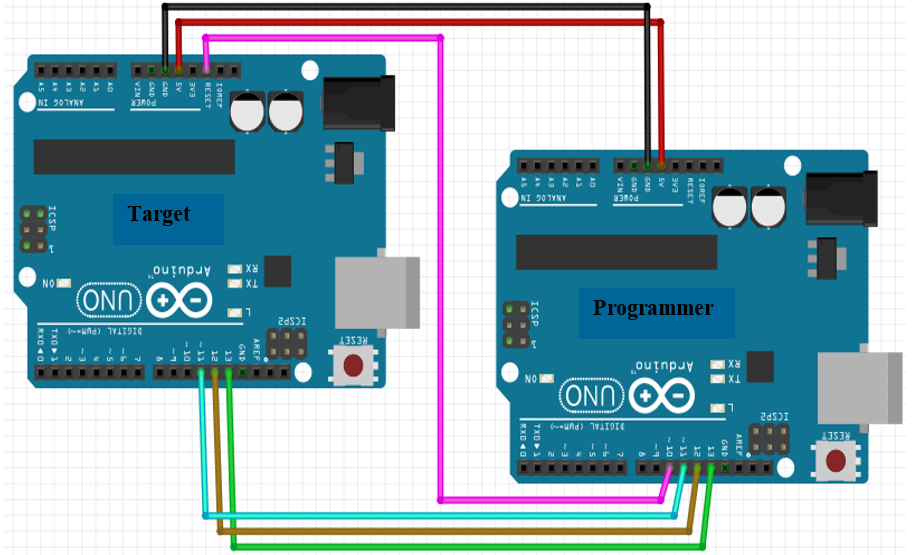
\includegraphics[scale=1.02]{EXP_16_Images/fig1.png}
\end{center}
\begin{center} {Figure 1. EasyEDA Workspace}\end{center}
  
Figure 1 is the workspace of EasyEDA and the navigation pane (left) is where we can find all our projects, files, parts, and footprints. After creating a new project, we can start making our schematic, as shown in figure 2.
\begin{center} 
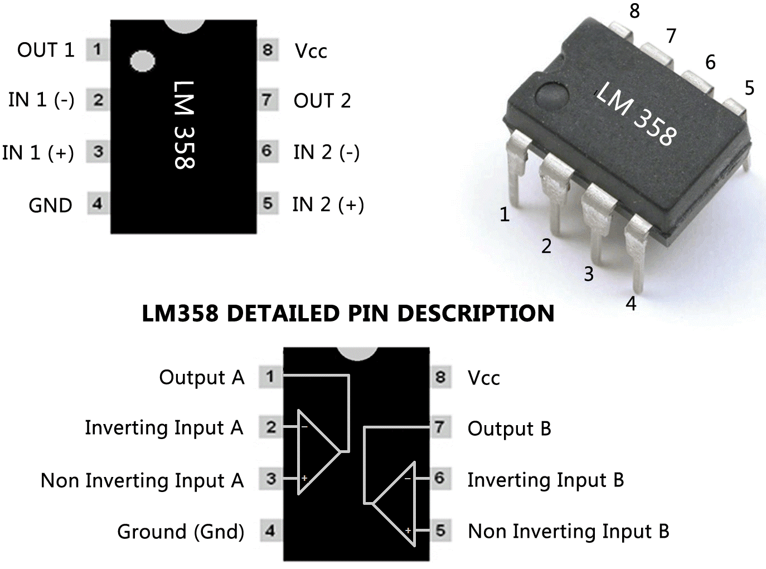
\includegraphics[scale=0.32]{EXP_16_Images/fig2.png}
\end{center}
\begin{center} {Figure 2. Schematic Editor}\end{center}
 
\vspace{13cm}
  
  \item Once we are done with the schematic design, we can then proceed to convert to PCB via Menu $>$ Design $>$ Convert to PCB
  
 \begin{center} 
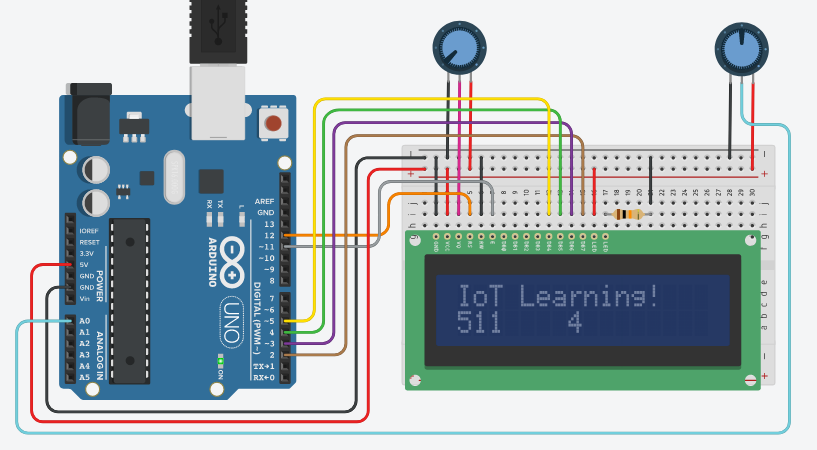
\includegraphics[scale=0.32]{EXP_16_Images/fig3.png}
\end{center}
\begin{center} {Figure 3. PCB Editor}\end{center}

  \item  Arrange the components on the PCB and then you can export GERBER files for manufacturing your PCB design via Menu $>$ Fabrication $>$ Gerber

  \item Upload your GERBER files on \href{https://jlcpcb.com/}{JLC PCB} and view your design.
\end{enumerate}

\\[14pt]
\noindent \textbf{\large PROCEDURE}\\[6pt]
We are going to design a PCB for the circuit diagram given in fig.4 and following are the steps to be followed:
\vspace{-6mm}
\begin{enumerate}
\setlength\itemsep{-0.3em}
\item Login or register on EasyEDA.
\item Make a new project and name it.
\item Create a new sheet.
\item Place components one by one, and connect them according to the schematic below.
\item Save the schematic.
\item Create a PCB file for your schematic.
\item Rearrange components to your desire.
\item Route the connections using both layers of PCB.
\item Save the PCB file.
\item Export GERBER files.
\end{enumerate}

Figure 5 shows the equivalent circuit diagram inside EasyEDA.

\begin{center} 
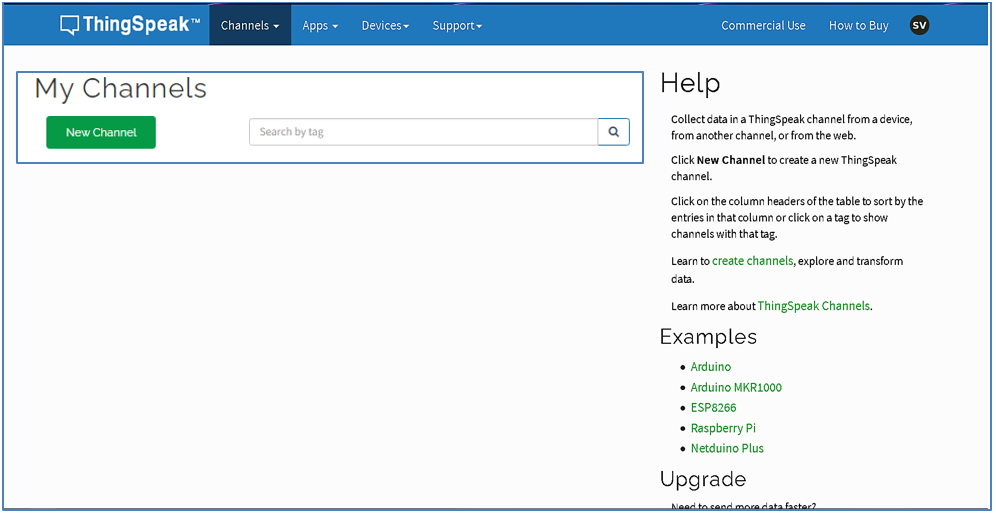
\includegraphics[scale=0.95]{EXP_16_Images/fig4.png}
\end{center}
\begin{center} {Figure 4. Circuit Diagram}\end{center}


\begin{center} 
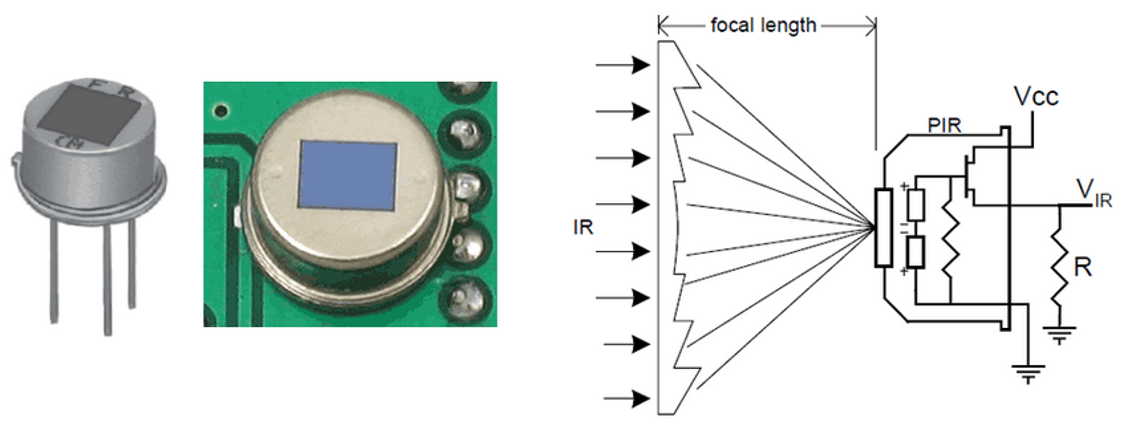
\includegraphics[scale=0.55]{EXP_16_Images/fig5.png}
\end{center}
\begin{center} {Figure 5.Schematic for ATMEGA328}\end{center}


\setlength{\parindent}{0eM}
\textbf{\large REFERENCE :}\\
\href{https://docs.easyeda.com/}{EasyEDA Documentation}\\ [9pt]
\noindent \textbf{\large CONCEPT DRILLS:}\\
Make a PCB design and export GERBER files.
\end{justify}
\end{document}